\documentclass[a4paper,11pt]{article}
\usepackage[utf8]{inputenc}
\usepackage[english]{babel} % Adds processing for some simple special characters.

% Packages for better page formatting and nice footnotes. %
\usepackage{fancyhdr} % Headers.
\usepackage{multicol} % Columns.
\usepackage[margin=0.75in]{geometry} % Margins.
\pagestyle{fancy}
\fancyhf{} % What does this do?
\lhead{Alexander S. Wheaton}
\rhead{\today}
\cfoot{\thepage}

% Title and author for title page. %

\title{Deep Stacking of AGN Hypervariables}
\author{
    Alexander S. Wheaton\\
    School of Physics and Astronomy\\
    The University of Edinburgh\\
    s1572046@ed.ac.uk\break
}

% Utilities for fine-grained control over image insertion. %

\usepackage{graphicx} % Insert images.
\usepackage{float} % Images float in document environment.
\usepackage{wrapfig} % Image/tables in multicols with \wrapfigure or \wraptable.
\usepackage{caption} % Captions for single images.
\usepackage{subcaption} % Captions for simultaneous images.
\graphicspath{ {./img/} }

% Not sure what this is for. %

\usepackage{fullpage,epsf}
\usepackage{lipsum}

% Some utilities for scientific and mathematical writing. %

\usepackage{siunitx} % Formatting for numbers with SI units.
\usepackage{amsmath} % Nice matrices.
% \usepackage{mathabx} % Astronomical symbols.
\usepackage{isotope} % Nice markup syntax for chemical symbols.
\usepackage{xfrac}   % Slant fractions and other utilities.

% Utilities for manual kerning adjustment. %

\newcommand\K{\kern.05em} % Small amount of kerning.
\newcommand\KK{\kern.1em} % Medium amount of kerning.
\newcommand\KKK{\kern.2em} % Large amount of kerning.
\newcommand\KKKK{\kern.3em} % Very large amount of kerning.

% Bibliography and referencing style.

\usepackage[backend=bibtex,style=phys,sorting=nyt]{biblatex} % Use style=draft for troubleshooting.
\addbibresource{references.bib}

% Page formatting.

\begin{document}

\thispagestyle{empty}                   % No numbers of title page
\epsfxsize=40mm                         % Size of crest
\begin{minipage}[b]{110mm}
    {\Huge\bf School of Physics\\ and Astronomy
    \vspace*{17mm}}
\end{minipage}
\hfill
\begin{minipage}[t]{40mm}
    \makebox[40mm]{
    \includegraphics[width=40mm]{crest.eps}}
\end{minipage}
\par\noindent                                           % Centre Title, and name
\vspace*{2cm}
\begin{center}
    \Large\bf \Large\bf Senior Honours Project\\
    \Large\bf Astrophysics\\[10pt]                     % Change to MP/CP/Astro
    \LARGE\bf Deep Stacking of AGN Hypervariables
\end{center}
\vspace*{0.5cm}
\begin{center}
    \bf Alexander S. Wheaton\\
    \today
\end{center}
\vspace*{5mm}

\begin{abstract}
    In this project, I examine the unusual luminosity of the galactic nucleus
    SDSS J094511 located at redshift $z=0.758$ using data gathered with the
    Liverpool Telescope on Las Palmas between 2012 and 2018. I develop several
    algorithms for centroiding on the object, for resampling to obtain higher
    resolution, and for stacking images to increase the S/N ratio in the frame.
    I extract radial and linear cross sections from the object and compare these
    to the point-spread-function of the Liverpool Telescope CCD to corroborate
    the hypothesis that linear increases in the luminosity over large timescales
    are \textit{not} due to instability of the viscous AGN accretion disk, but a
    gravitational microlensing event by a star in an intervening galaxy or dwarf
    galaxy.
\end{abstract}

\vspace*{1cm}

\subsubsection*{Declaration}
\begin{quotation}
    I declare that this project and report is my own work.
\end{quotation}

\hspace*{1cm}Signature:\hspace*{1cm}\includegraphics[width=6cm]{signature_repaired.eps}\hspace*{1cm}Date: \today

\vfill
\noindent{\bf Supervisor:} Professor A. Lawrence, FRSE, FRaS
\hfill
12 Weeks

\newpage
\setcounter{page}{1} % Set page number to 1
\tableofcontents

\newpage
\section{Introduction}\label{sec:introduction}

The luminosity of most galaxies is dominated by stellar emission and emission
from hot gas and dust in the interstellar medium, which is heated by their constituent stars. As such, it is mostly confined to the wavelength range of typical stars---the ultraviolet through the infrared. Between 1--50\% of galaxies in the local universe, however, show strong emission in a wider range of bands, from gamma rays to the radio spectrum. The source of these emissions is typically confined to a compact nuclear region, and such objects are therefore called active galactic nuclei (AGN).\cite{mcclure_2019}

AGN are distinguished from one another by their luminosities, spectra, and
ratio of nuclear to galactic luminosity into four main groups: Seyfert galaxies,
quasars, radio galaxies, and optically-violent variables. The aforementioned
properties vary among these broad catagories, but most AGN exhibit several characteristics which are relevant to this project\cite{mcclure_2019}:

\begin{itemize}
    \item a luminous and compact appearance
    \item a broad spectral energy distribution which is not explicable by thermal(blackbody) emission
    \item variable luminosity over short timescales of minutes to days
\end{itemize}

\subsection{The Viscous Accretion Disc}\label{sec:viscous_accretion_disk}

The underlying mechanism for this luminosity is widely understood to be the accretion of matter onto a supermassive black hole.\cite{mcclure_2019} The luminosity, compactness and sprectra of AGN are well described by a model in which matter that falls into a black hole with some amount of angular momentum, forming an accretion disk. Gravitational potential energy is changed for kinetic energy (and therefore angular momentum), and viscous processes between particles on different orbits create drag, transferring angular momentum outward and heating the disk. This energy is then radiated thermally.\cite{lawrence_2018}

Small adjustments to this model for surrounding clouds and ``atmosphere'' closely fit observed spectral energy distributions.\cite{lawrence_2018}. What this model fails to explain, however, is the extreme variability of AGN. A viscosity parameter which explains observed luminosities should also result in a very stable disk, for which changes in the optical spectrum take place only on the order of $10^3$ years.\cite{lawrence_2018}

The accretion disk model was briefly rescued by the idea of X-ray reprocessing, but recent observations of ``hypervariable,'' high-luminisity AGN by the Sloan Digital Sky Survey (SDSS), the Panoramic Survey Telescope and Rapid Response System (Pan-STARRS) have once again cast uncertainty onto the model.\cite{lawrence_2018} These objects vary on timescales comparable to the time for information to propagate over the Scharzchild radius of a supermassive black hole\cite{mcclure_2019}\cite{lawrence_2018}:

\begin{equation}
    \Delta t \geq \frac{R_{Sch}}{c} = \frac{2GM}{c^3}
\end{equation}

\noindent That such extreme changes should happen on these timescales and in the optical spectrum suggests that the disk undergoes incredible physical change and that this change propagates relativistically through the disk---a strong argument for instability.

\subsection{The Pan-STARRS Survey}\label{sec:panstarrs_survey}

In 2016 Lawrence et. al identified fifteen transiently luminous, blue AGN in the Pan-STARRS1 Survey by comparison with earlier data from the SDSS. These targets were subsequently monitored with the Liverpool Telescope (LT) on Las Palmas, and found to be hypervariable AGN over timescales of several years.\cite{lawrence_2016}

\begin{figure}[h!]
    \centering
    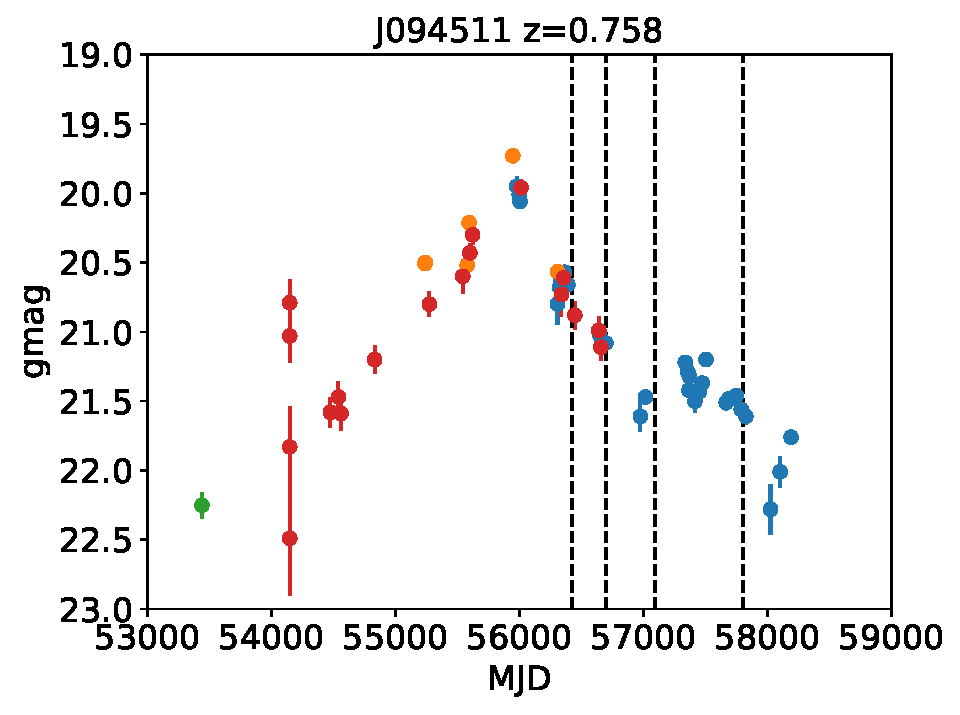
\includegraphics[width=0.67\textwidth]{J094511_magnitudes.eps}
    \caption{Magnitude of SDSS J094511 from SDSS, CRTS, PanSTARRS, and LT observations, over ten years.}
    \label{fig:magplot}
\end{figure}

One such transiently luminous, blue hypervariable AGN is SDSS J094511, an object in the constellation Leo and at redshift $z=0.758$.\cite{lawrence_2016}\cite{bruce_2017} Fig. \ref{fig:magplot} shows the evolution of magnitide of J094511 in the Sloan $g'$ band between 2004 and 2014, using combined data from the SDSS, from the Catalina Real-Time Transit Survey (CRTS), from Pan-STARRS1, and the LT. The object evolves at $\sim 0.4 $ mag/yr from $g' \sim 22.2$ to $19.7$ and back again, during which time its luminosity changes by a factor of $\sim 2$.\cite{bruce_2017}. This magnitude of evolution over a period of ten years is not explicable by the accretion disk model alone.

Lawrence et. al (2016) therefore propose several possible explanations for these events, with the most likely candidates being i) changes in the accretion state of the disk (i.e. matter falling into an otherwise quiet AGN) and ii) gravitational lensing events by stars in intervening galaxies or dwarf galaxies.\cite{lawrence_2016} Lensing is a well established explanation for AGN variability, and can take the form of either macro-lensing due to the gravitational potential of the entire intervening galaxy or microlensing by a single or few constituent stars. The latter event is more likely to be the case for small galaxies, for which the macroscopic gravitational potential does not dominate the lensing effect.\cite{lawrence_2016}

 There are several signatures which may indicate that this is the case for a particular object. If the AGN is modeled as point source and intervening star modeled as a lens (henceforth: simple microlensing model), it is possible to compute the lightcurve $F(t) = \mu(t)F_s$ which describes the evolution of the lensed AGN with respect to its unlensed flux, as described by Bruce et al. (2017). This model contains seven free parameters, one of which is a flux contribution $F_b$ from the host galaxy of the lensing star(s). Although a simplification, this model is particularly useful for understanding hypervariables like J094511, whose light curves evolve smoothly.\cite{bruce_2017}

 The parameter $F_b$ is key to demonstrating a lensing event, as background flux may be detectable in the cross sectional luminosity curve of the object. In this project, I develop methods for quantifying this parameter by stacking frames from the Liverpool Telescope to improve signal to noise ratio and depth of field, and for extracting the luminosity profile of objects in the frame for comparison to the point spread function of the Liverpool Telescope.

\section{Liverpool Telescope Data}

There are several technical problems associated with the LT data. In many frames, astronomical seeing is very poor. All frames, particularly in the Sloan $u'$-band, are littered with cosmic ray detection events. Each of these factors obfuscates the already faint luminosity profile of J094511, and I have employed several statistical methods to mitigate them.

\subsection{Stacking to Increase S/N Ratio}

For astronomical frames in which the noise is background limited (i.e. thermal, source, and read noise are negligible compared to the sky) the signal to noise ratio goes as\cite{lawrence_2014}\cite{mcclure_2019}:

\begin{equation}
    \frac{S}{N} = \frac{n_\star t}{\sqrt{n_{pix}n_st}} \propto t^{\sfrac{1}{2}}
\end{equation}

Where $t$ is the exposure time of the frame. S/N ratio increases with exposure time, although with diminishing marginal returns. Very long exposures, however, are typically limited by the saturation point of the CCD. A typical approach to increasing the S/N ratio of observations, then, is to ``stack'' the frames of many short exposures, summing up the counts recieved at each point in the sky in each frame.\cite{mcclure_2019} As the S/N ratio increases, faint objects in the frame like J094511 become more distinguishable from the background (increased depth of field), and cosmic ray detections disappear into the background, both without saturating the CCD.

\subsection{Astronomical Seeing}\label{sec:astronomical_seeing}

Atmospheric turbulence creates a differential density of air above ground-based telescopes, distorting light wavefronts and obfuscating astronomical objects with ``speckles.'' This phenomenon is called atmospheric seeing, and is typically quantified by $\theta_s$, the hypothetical full width at half maximum of an ``airy disc'' which distorts incoming wavefronts.

\begin{figure}[h!]
    \includegraphics[width=0.32\textwidth]{seeing_hist_U_band.eps}
    \includegraphics[width=0.32\textwidth]{seeing_hist_G_band.eps}
    \includegraphics[width=0.32\textwidth]{seeing_hist_R_band.eps}
    \caption{Astronomical seeing of the LT data in Sloan \textit{u'g'r'} bands.}
    \label{fig:seeing}
\end{figure}

Astronomical seeing values of $\theta_s=1''$ are typical for optical wavelengths, where the Sloan bands lie. Values below this are considered exceptionally good seeing.\cite{mcclure_2019}\cite{lawrence_2014} It is desirable to discard frames with higher seeing values, but this must be balanced against the need for additional frames to increase the S/N ratio in the final stack. Fig. \ref{fig:seeing} shows the distribution of seeing values, in arcseconds, in each of the Sloan \textit{u'g'r'} bands, with the mean (blue) and standard deviations (red) plotted vertically. It is clear that discarding frames with $\theta_s>1''$ would result in substantially reduced dataset, and a resultingly low S/N ratio for an already faint object. For this reason, I have elected to discard all frames for which $\theta_s>\bar{\theta_s}+\sigma_\theta$, where the seeing parameter is more than one standard deviation above the mean parameter. This includes most of the available data in each band, while exluding the worst seeing parameters. It is also a more rigorous and reproducible approach to ensuring the best possible stack.

A single image of J094511 in the $u'$-band has a seeing of $r_0=999.0''$, which is likely an error or the result of exceptional atmospheric turbulence. Including this value in the statistics derived from the seeing distribution would badly skew $\bar{\theta_s}$ and $\sigma_\theta$. For this reason, the image has been discarded and its seeing parameter excluded from the calculation of the mean and standard deviation of the seeing distribution.

\subsection{FITS World Coordinate Data}

Finally, individual frames in the dataset are not all centered on the same equatorial coordinates, and must therefore be aligned before they can be stacked. Individual frames are stored using the NASA FITS standard, which contains a series of header data units (HDUs), each of which contain a data cube and metadata associated with that cube.\cite{FITS_standard} The LT HDUs contain a single, 2-dimensional arrays of counts per pixel for each frame. The metadata of each HDU contains the astronomical seeing, roation, and crucially, the World Coordinate System (WCS) associated with each frame.\cite{greisen_2002} The WCS data contains several key pieces of information for aligning individual frames.

\begin{table}[h!]
    \centering
    \begin{tabular}{ | l | c | l |} \hline
        Header Key & Value & Meaning \\ \hline \hline
        CTYPE1  & 'RA---TAN'     & Coordinate projected onto x-axis \\
        CTYPE2  & 'DEC--TAN'     & Coordinate projected onto y-axis \\
        CRPIX1  &  512.          & WCS reference pixel coordinate \\
        CRPIX2  &  512.          & WCS reference pixel coordinate \\
        CRVAL1  &  146.295274426 & [degrees] World coordinate at the ref pix \\
        CRVAL2  &  17.76338016   & [degrees] World coordinate at the ref pix \\
        CDELT1  & -7.7508973E-05 & [degrees/pixel] Platescale along x-axis \\
        CDELT2  & 7.7508973E-05  & [degrees/pixel] Platescale along y-axis \\
        CROTA1  & 90.361783      & [degrees] Rotation of xy-axes w.r.t. east-north \\
        CROTA2  & 90.361783      & [degrees] Rotation of xy-axes w.r.t. east-north \\ \hline
    \end{tabular}
    \caption{\label{tab:FITS_header}Example FITS header keys and values from the LT.}
\end{table}

While the WCS projection and platescale (CDELT1/CDELT2) are constant across all frames, other WCS values---most importantly the world coordinate at the reference pixel---vary from frame to frame. Random frames are rotated by multiples of $\sfrac{\pi}{4}$ from the $(x,y) \rightarrow (-\alpha, \delta)$ mapping. Additionally, frames taken after 2014 have twice the field of view of previous frames, with a reference pixel of (1024,1024), rather than (512,512). There are also systematic errors in the $(\alpha, \delta)$ coordinate of the reference pixel (see Sec. \ref{sec:wcs_centroid}).

\section{The \textsc{AstroPy} and \textsc{FITS-Utils} Modules}

To correct for these factors, I utilised the \textsc{AstroPy} module for \textsc{Python 3.5.2}. The \textsc{AstroPy} module allows one to load in FITS compliant files as HDU objects which contain all the data and metadata associated with a particle file. Performing math on the data stored in these objects, however, can modify the original FITS file\cite{astropy_2013}\cite{astropy_2018}, so I modified and extended the functionality of the \textsc{fits-utils} module, written for aligning and stacking on the Telescope Group Project course at the University of Edinburgh.\footnote{\url{github.com/aswheaton/fits-utils}} HDU data cubes are loaded into \textsc{NumPy} arrays and stored in an ``image-dictionary''. Relevant metadata for each image are also stored in this dictionary, which behaves similarly to the \textsc{AstroPy} HDU object.

I then algorithmically sort frames by seeing value according to the standards defined in Sec. \ref{sec:astronomical_seeing}, rotate each array if necessary so that $(x,y) \rightarrow (-\alpha, \delta)$, crop the array if necessary to 1024x1024 pixels, and reassign the coordinates of reference pixel to (512,512) if the array is cropped. The image-dictionaries are then ready to be aligned and stacked.

\section{Centroiding on J094511}

In order to align each image, its offset, in pixels, with respect to every other image in the stack must be determined. The location of J094511 varies around the reference pixel in each frame, and the relative offset of each image can be computed by comparing the location of the object in each.\footnote{Note that from here on, the phrases ``pixel coordinates'' or ``image coordinates'' will be used to refer to the $(x,y)$ coordinates of pixels in the image, which are mapped to $(-\alpha,\delta)$ as defined by the FITS file standard\cite{FITS_standard}. The phrase ``array coordinates'' will be used to refer to the $(row,column)$ indices of the \textsc{NumPy} array containing the image. This is an important distinction, as pixel coordinates are mapped to array coordinates by $(x,y) \rightarrow (column, row)$.}

Determining the precise location of the object, however, is a non-trivial task. J094511 has a spread of $\sim10$ pixels in each frame. A naive approach to determining its centerpoint would be to take the pixel coordinates of the maximum value of the object, but doing this algorithmically quickly proves futile and innaccurate. J094511 is by far one of the faintest objects in the frame, and there is no obvious way to distinguish pixels which contain the object from pixels which do not. Even a hard coded cutout from the array, which was manually verified to always contain the object, frequently contains sufficient noise and cosmic ray events to confuse any maximum value finding algorithm. Even if this were possible, poor atmospheric seeing distorts the object so that the brightest pixel is commonly \textit{not} at the center of the object (dubiously assuming that the ``above atmosphere'' brightest pixel is even at the center, or the same across frames).

\subsection{Two Dimensional Weighted Mean}\label{sec:flux_weighted_mean}

A better method for computing the centroid of the object is to calculate the flux weighted mean in two dimensions:

\begin{equation}
        (\bar{x},\bar{y}) =
        \left( \frac{1}{n_{tot}} \sum_{i}^{} n(x_i) x_i,
        \frac{1}{m_{tot}} \sum_{j}^{} m(y_j) y_j \right)
\end{equation}

\noindent Whereby all the counts are first summed along the $y$-axis and the flux weighted mean of position, $\bar{x}$, calculated, and then the inverse---summing along the $x$-axis and calculating $\bar{y}$---is performed. This is a more reliable method of calculating the object centroid, which tends to downweight individual speckles from atmospheric seeing and cosmic ray events. Unfortunately, performing a 2D weighted mean on the entire frame invariably yields the reference (center) pixel coordinates for $(\bar{x},\bar{y})$. No source in the LT frames is sufficiently bright to reliably pull this average away from the center pixels, even when rescaled exponentially. Least of all is J094511 able to do this.

The weighted average calculation, it turns out, is only sensitive to objects which nearly fill the sample region. There is enough variation in the location of J094511 between frames that a hard coded cutout from the array which will always contain the object is large enough to suffer the same problem. A smaller cutout region is need. Thus, a technique for accurately and algorithmically making an initial guess at the location of the object, around which a small cutout region can be made dynamically, was developed using the WCS data from the LT FITS headers.

\subsection{Initial Guess: WCS Centroiding}\label{sec:wcs_centroid}

By comparing the known coordinates of J094511, ($\alpha$,$ \delta$) = (9:45:11.08,+17:45:44.78) to the world coordinates at the reference pixel, we can compute an initial guess for the location of J094511. Some trivial linear algebra gives that:

\begin{align}
    x_\star = p_\alpha(\alpha_\star - \alpha_{ref}) + x_{ref} \\
    y_\star = p_\delta(\delta_\star - \delta_{ref}) + y_{ref}
    \label{eq:wcs_linalg}
\end{align}

\noindent Where $(x,y)$ are pixel coordinates, $(\alpha,\delta)$ are equatorial coordinates in degrees, $\star$ denotes values associated with the object of interest and $ref$ denotes values associated with the reference pixel. The values $p_\alpha$ and $p_\delta$ are the platescale values from the FITS header, corresponding respectively to keys CDELT1 and CDELT2 in Table \ref{tab:FITS_header}.

In developing this method, however, I found that the LT WCS data is consistently off by $\sim25$ pixels along the $x$/$\alpha$-axis, or about $7''$. This is easily corrected by an extra term in Eq. \ref{eq:wcs_linalg}, so I wrote the WCS centroiding function to accommodate a user specified correction factor.

Once corrected, the pixel coordinatess of the intitial guess are rounded to the nearest whole pixel, mapped back to array coordinates and a cutout of 10x10 pixels taken around them. I perform the weighted mean calculation for this smaller array, round the result to the nearest whole pixel value, and map this centroid back to the array coordinates of the entire image.

This process produces reasonably good centroid values in almost every frame, but has some disadvantages. First, there are two points in the process where a non-integer pixel coordinate is necessarily rounded: once when calculating the offset from the reference pixel, and again after performing the weighted mean. Each of these introduce an error into the centroid calculation. For larger objects, this might be negligible, but for objects such as J094511 which are scarcely 10 pixels across on the LT CCD, each error of $\pm0.5$ pixels is considerable. Second, this approach still limits centroid resolution to the number of pixels in the objects' footprint on the CCD, while the true centroid is, of course, not guaranteed to be at an integer pixel value in any frame.

Once these centroid values are obtained, I carry out the alignment of each frame and stack them accordingly. This process is elaborate, and will only be described in summary here.\footnote{Full implementation of the algorithm at \url{github.com/aswheaton/lt-stacking-project}.} First, the maximum displacements in array coordinates $\Delta r_{max}$ and $\Delta c_{max}$ are calculated from all the centroid values in the stack. These values are used to create an array of zeros, with dimensions $(1024+\Delta r_{max})$x$(1024+\Delta c_{max})$, which are sufficient to hold all the images, once aligned. For each image, then, the displacement in array coordinates with respect to the \textit{minimum} centroid values in the stack, $r_{min}$ and $c_{min}$, and these values, $\Delta r$ and $\Delta c$ are used to cast the unaligned image into its aligned position in the array of zeros. This is done such that:

\begin{equation}
    (r_{align}, c_{align}) = (r_{unalign} + \Delta r, c_{unalign} + \Delta c)
\end{equation}

\noindent For each pixel in the array. The resulting stack of aligned images is summed and the resulting array saved to a new image dictionary. This produces a much better defined object, as shown in Fig. \ref{fig:wcs_centroids}. By fitting a two dimensional Gaussian to this data, I begin to quantify the properties of J094511 and the sky background on which it lies. Table \ref{tab:wcs_gaussians} shows the fitted parameters for the resulting stack in each of the Sloan $u'g'r'$ bands.

\begin{figure}[t]
    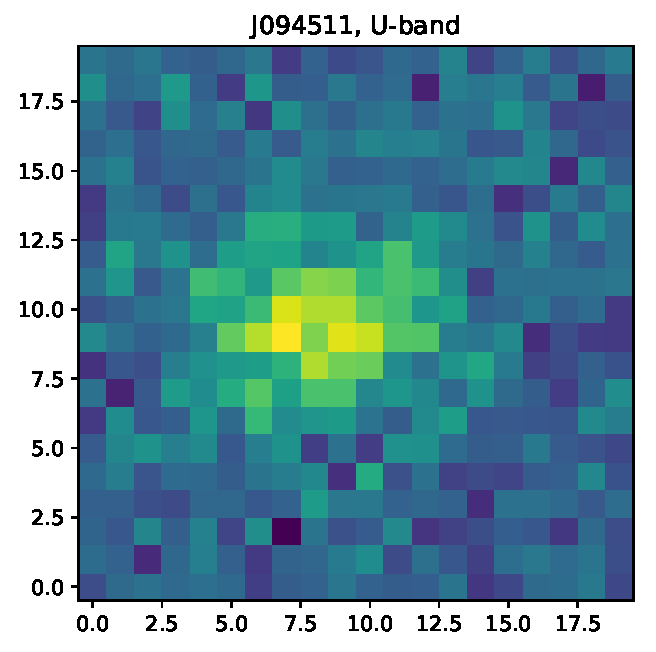
\includegraphics[width=0.32\textwidth]{wcs_centroid_U_stack.eps}
    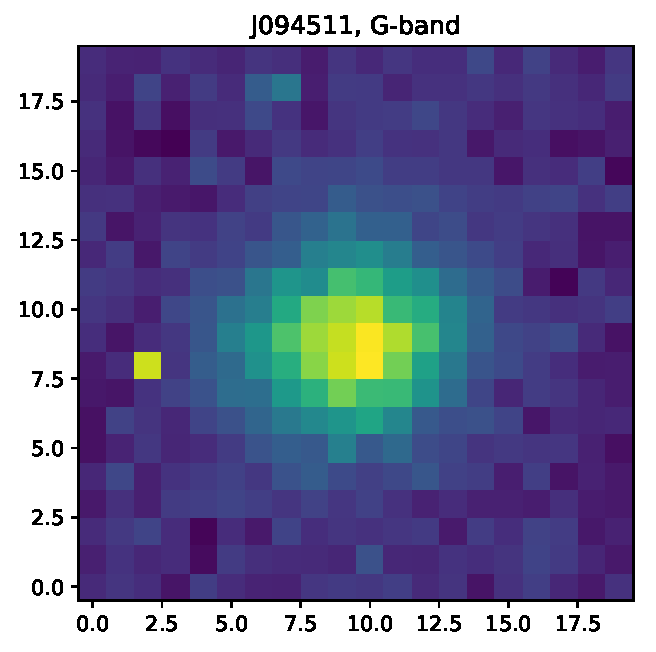
\includegraphics[width=0.32\textwidth]{wcs_centroid_G_stack.eps}
    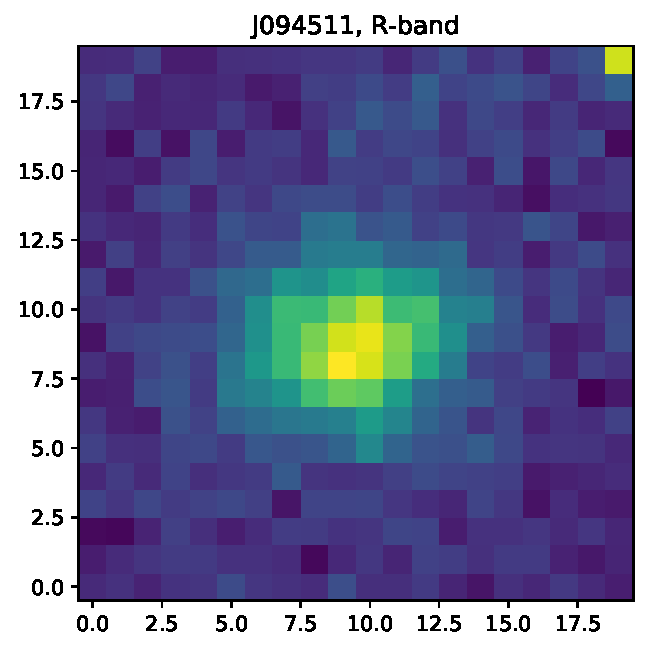
\includegraphics[width=0.32\textwidth]{wcs_centroid_R_stack.eps}
    \caption{Image stack of J094511 in the Sloan $u'g'r'$ bands.}
    \label{fig:wcs_centroids}
\end{figure}

\begin{figure}[t]
    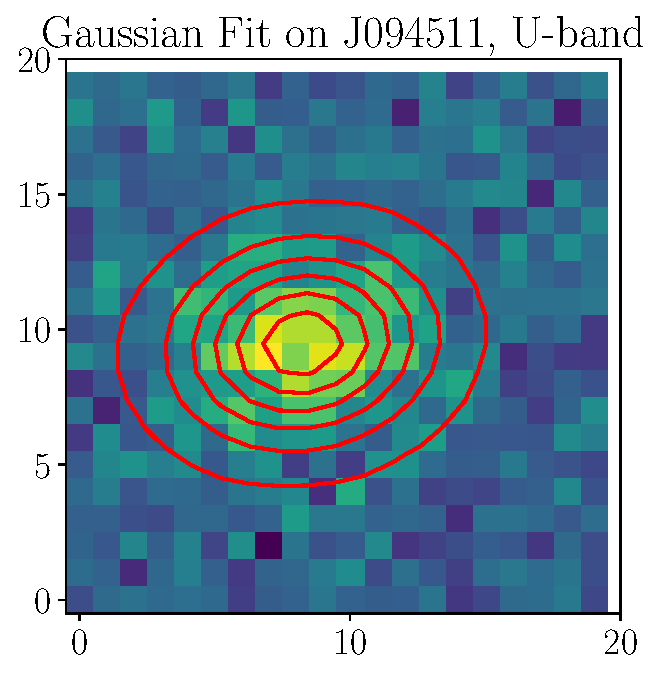
\includegraphics[width=0.32\textwidth]{gauss_fit_wcs_U_stack.eps}
    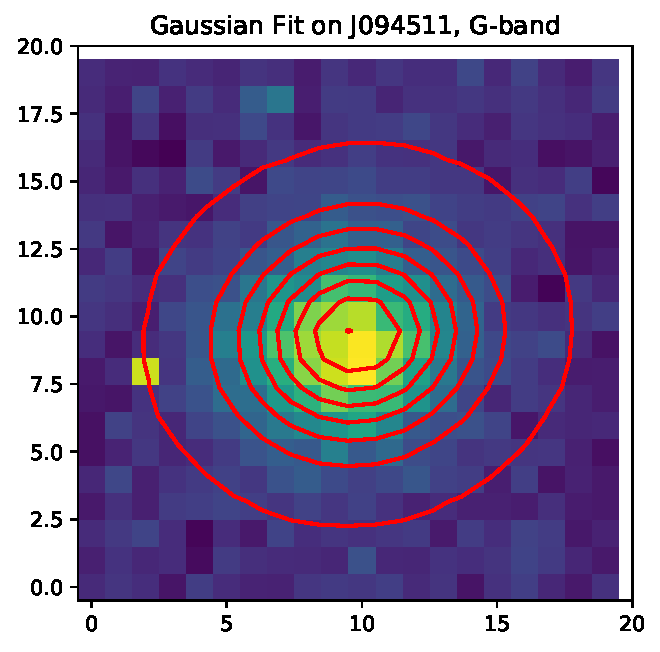
\includegraphics[width=0.32\textwidth]{gauss_fit_wcs_G_stack.eps}
    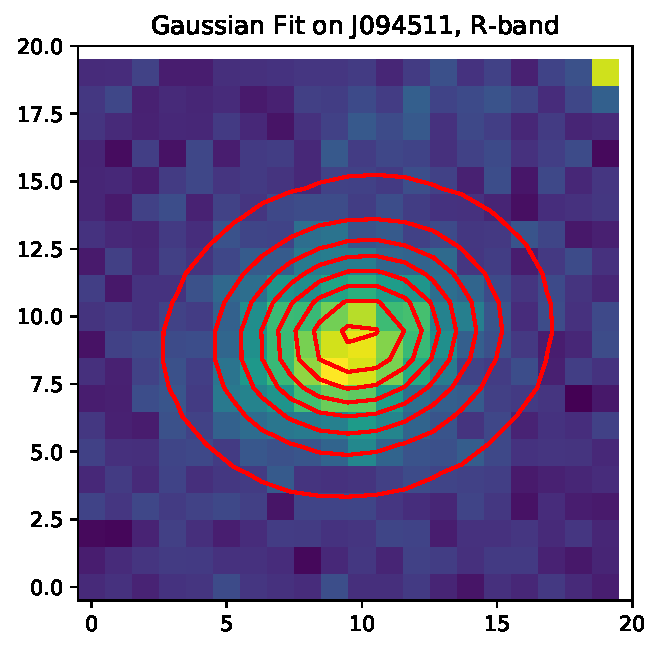
\includegraphics[width=0.32\textwidth]{gauss_fit_wcs_R_stack.eps}
    \caption{Gaussian fit on J094511 in the Sloan $u'g'r'$ bands.}
    \label{fig:gauss_fit_wcs_stack}
\end{figure}

\begin{table}[h!]
    \centering
    \begin{tabular}{| c | c | c | c | c | c | c |} \hline
        Band & Amplitude & $x_0$ & $y_0$ & $\sigma_x$ & $\sigma_y$ & $\theta$ \\ \hline \hline
        $u'$ & $250(10)$ & $8.2(2)$ & $9.5(1)$ & $0.83(4)''$ & $0.64(3)''$ & $0.2(1)$ \\
        $g'$ & $2170(50)$ & $9.34(6)$ & $8.85(5)$ & $0.75(2)''$ & $0.66(2)''$ & $0.2(1)$  \\
        $r'$ & $2270(60)$ & $9.37(7)$ & $8.81(6)$ & $0.75(2)''$ & $0.60(2)''$ & $0.02(1)$ \\ \hline
    \end{tabular}
    \caption{Fitted Gaussian parameters for WCS based stacking.}
    \label{tab:wcs_gaussians}
\end{table}

Amplitude is given in counts, and is measured with respect to the background. The parameters $(x_0,y_0)$ are given in pixel coordinates of the cutout, and their promimity to the central pixel value 9.5 can be used to quantify the ``goodness'' of the original centroids. $\sigma_x$ and $\sigma_y$ are given in arcseconds, and $\theta$ in radians.

\subsection{Refinement: Gaussian Fitted Centroiding}

Gaussian fitting, however, presents a solution to some of the shortcomings of the flux weighted mean centroid described in Sec. \ref{sec:flux_weighted_mean}. Once a Gaussian function is fitted to the existing data, the fitted parameters can be used to interpolate the number of counts at non-integer pixel values. This is called resampling, and can be used to obtain a 2D profile of the object with ``infinite'' resolution.

Gaussian fitting is also another way to determine the centroid $(x,y)$ of each unaligned image. In two dimensions, the power to which $e$ is raised in the Gaussian function is any negative-definite quadratic form. The contour lines of a Gaussian will therefore always be elipses.\cite{astropy_gaussian} The functional form of the two-dimensional Gaussian is:

\begin{equation}
    f(x,y) = A \exp\left(- \left(\frac{(x-x_0)^2}{2\sigma_x^2} + \frac{(y-y_0)^2}{2\sigma_y^2} \right)\right)
\end{equation}

\noindent Where $A$ is the amplitude, $(x_0, y_0)$ are the center in pixel coordinates, $\sigma_x$, $\sigma_y$ are the spread of Gaussian in the $x$ and $y$ directions.\cite{wolfram_gaussian} Generally, a two-dimensional elliptical Gaussian function is expressed as:

\begin{equation}
    f(x,y) = A \exp\left(- \left(a(x - x_0)^2 + 2b(x-x_0)(y-y_0) + c(y-y_0)^2 \right)\right)
\end{equation}

\noindent The coefficients:

\begin{align}
a & = \frac{\cos^2\theta}{2\sigma_x^2} + \frac{\sin^2\theta}{2\sigma_y^2} \\
b & = \frac{\sin2\theta}{4\sigma_x^2} - \frac{\sin2\theta}{4\sigma_y^2} \\
c & = \frac{\sin^2\theta}{2\sigma_x^2} + \frac{\cos^2\theta}{2\sigma_y^2}
\end{align}

Allowing one to specify a counterclockwise angle $\theta$.\cite{astropy_gaussian} The \textsc{SciPy} module uses the least squares method to fit values to each of these six free parameters\footnote{In order for fit these parameters, the \textsc{SciPy} module requires an initial guess.\cite{scipy_module_2020} I tested two approaches to devising this guess algorithmically. The first is to use statistics of the cutout as the initial guess: the background (median) subtracted maximum as the amplitude, the flux weighted mean described in Sec. \ref{sec:flux_weighted_mean} as $x_0$, $y_0$, and the median for the offset. The other approach is to use the fitted parameters from Table \ref{tab:wcs_gaussians}, since these are fitted to a profile with a much higher S/N ratio than the individual frames. As it turns out, both these approaches produce very similar results.}, $A$, $x_0$, $y_0$, $\sigma_x$, $\sigma_y$, $\theta$, and an offset.\cite{scipy_module_2020} The parameters $(x_0, y_0)$ are then the centroid of the object in array coordinates. I do this for each unaligned frame in the stack, and then for all frames, set $x_0$ and $y_0$ to zero to align them. (If the rotation of frames from the LT varied, it would also be necessary to set $\theta$ to zero).

\begin{figure}[h!]
    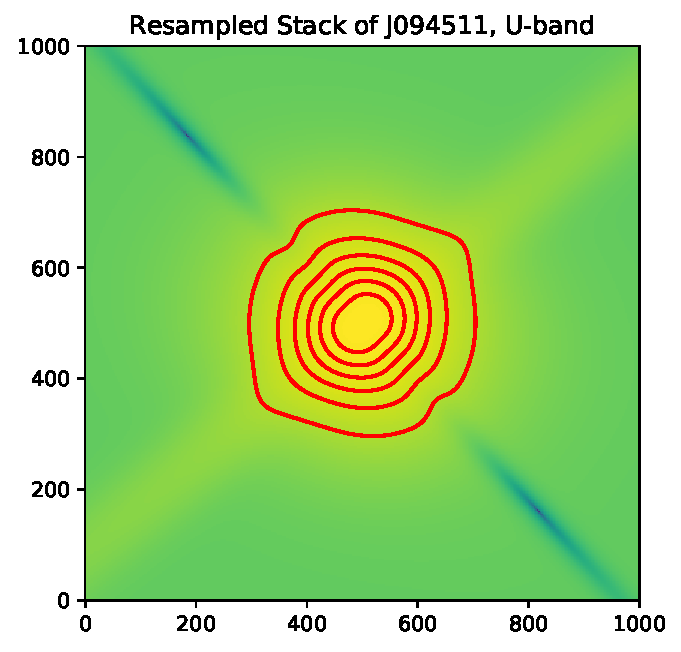
\includegraphics[width=0.32\textwidth]{J094511_U_resampled_stack.eps}
    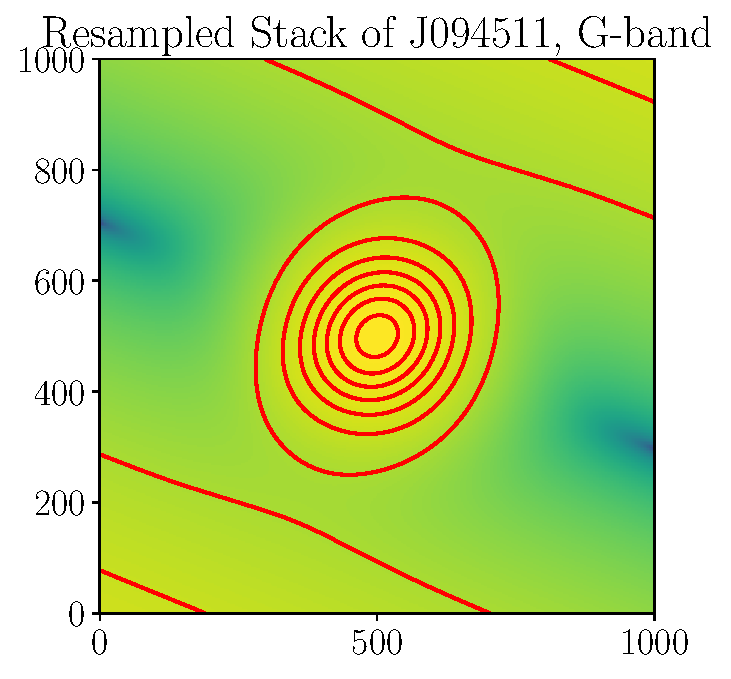
\includegraphics[width=0.32\textwidth]{J094511_G_resampled_stack.eps}
    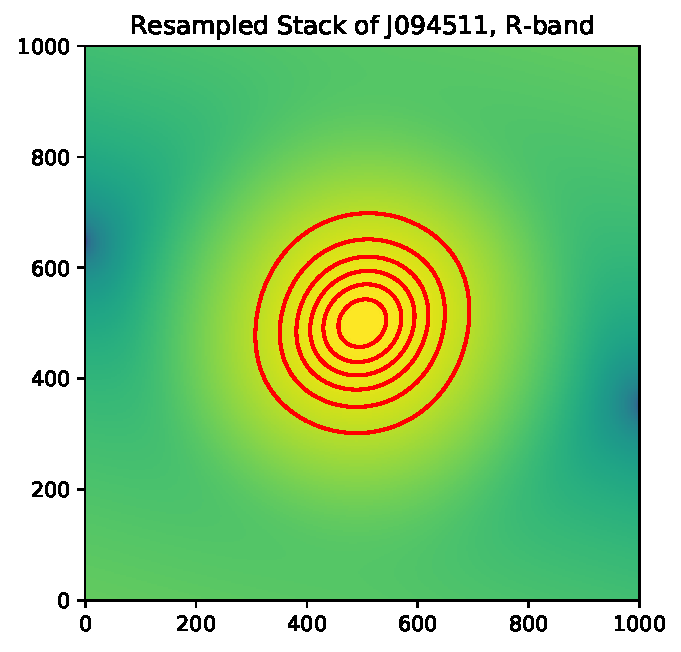
\includegraphics[width=0.32\textwidth]{J094511_R_resampled_stack.eps}
    \caption{Resampled stacks of J094511 in the Sloan $u'g'r'$ bands, at increased resolution.}
    \label{fig:resampled_stacks}
\end{figure}

I now have a smooth function for the profile, in two dimensions, of the the object in each frame, and I can sample values from this profile at any non-integer pixel coordinate. The resolution of the cutout around J094511 is therefore scaled up from 20x20 pixels to 1000x1000 pixels, values sampled from the coordinate at each pixel, and each column in the stack summed as described in Sec. \ref{sec:wcs_centroid}. The resulting stacks are shown in Fig. \ref{fig:resampled_stacks}, at much higher resolution than is achievable by stacking whole pixels from the LT frames.

I can once again fit a Gaussian to these stacks to quantify the properties of the object (we know indeed that it must have a Gaussian form, because it is a linear combination of Gaussians I have already fitted). Fitted parameters for the resampled stack are listed in Table \ref{tab:resampled_gaussians}.

\begin{table}[h!]
    \centering
    \begin{tabular}{| c | c | c | c | c | c | c |} \hline
        Band & Amplitude & $x_0$ & $y_0$ & $\sigma_x$ & $\sigma_y$ & $\theta$ \\ \hline \hline
        $u'$ & $385.42(5)$ & $499.50(1)$ & $499.50(1)$ & $0.5681671(8)''$ & $0.5253415(8)''$ & $0.689(1)$ \\
        $g'$ & $2889.0(2)$ & $499.500(6)$ & $499.500(5)$ & $0.6119158(4)''$ & $0.5567006(3)''$ & $3.9696(4)$ \\
        $r'$ & $3168.9(2)$ & $499.500(6)$ & $499.500(6)$ & $0.5290998(4)''$ & $0.5792824(4)''$ & $2.4727(5)$ \\ \hline
    \end{tabular}
    \caption{Fitted Gaussian parameters for resampled stacking.}
    \label{tab:resampled_gaussians}
\end{table}

\noindent These parameters are similar to the values obtained for whole pixel stacking of the LT frames, but describe a slightly more compact source. They are also derived from a stack with much higher resolution, so their errors are appropriately smaller. Here, it is worth noting that the errors on these values are really errors on the fit. Indeed, it is not sensible that we should be able to determine the spread of an object to the nearest ${10^{-7}}''$, when the atmospheric seeing of the frames from which the fit is derived are on the order of $1''$. There is considerable variation in the fitted value of $\theta$ across bands, but since this stack is less elliptical than the whole pixel stack, the covariance of $\theta$ with other parameters in the fit is small, and any rotation value will likely fit the data well. Interestingly, the resampled and stacked image of the object is slightly redder than its whole pixel counterpart. Further investigation is needed to determine why this is the case.

It is tempting to ascribe the two-lobed appearance of the object in the $u'$ band to the geometry of the AGN (as this is indeed one of their possible geometries) but those emissions are typically in the radio region, and it is more likely that this is due to greater variance in $\sigma_x$ and $\sigma_y$ in the $u'$ band.

\section{Radial Cross Sections of J094511}

With this new profile, we can begin to make meaningful statements about $F_b$, the flux contribution from the host galaxy of the lensing star(s), described in Sec. \ref{sec:panstarrs_survey}. By summing up the number of counts in annuli of increasing radius around the object and dividing by the area of each annulus, I extract a 1D, radial profile of the flux from J094511, shown in Fig. \ref{fig:radial_profiles}.

\begin{figure}[h!]
    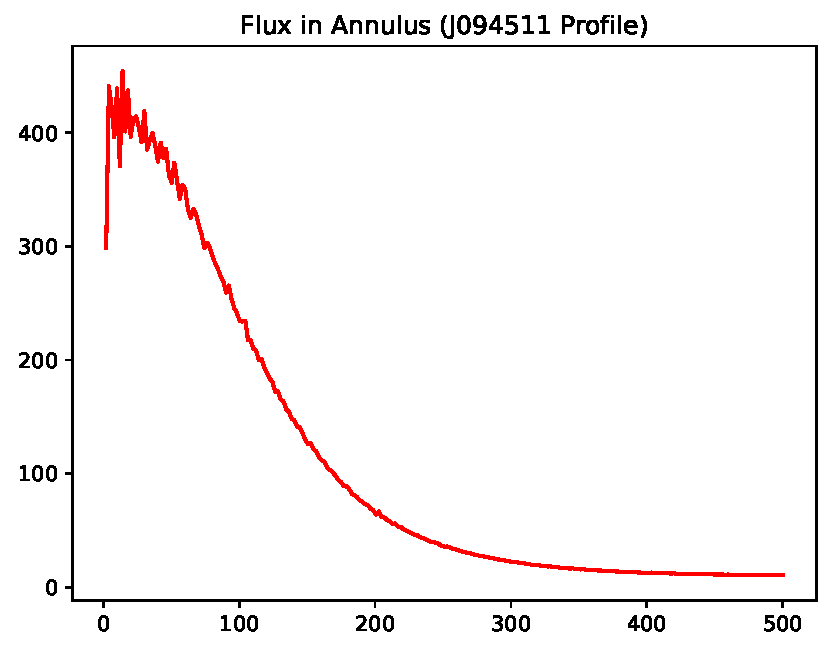
\includegraphics[width=0.32\textwidth]{J094511_U_annulus_flux.eps}
    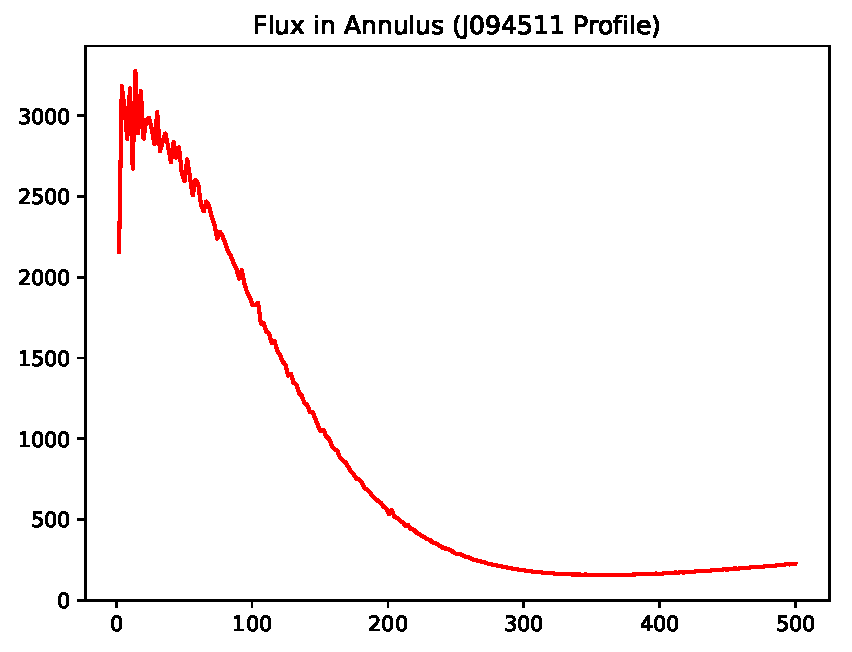
\includegraphics[width=0.32\textwidth]{J094511_G_annulus_flux.eps}
    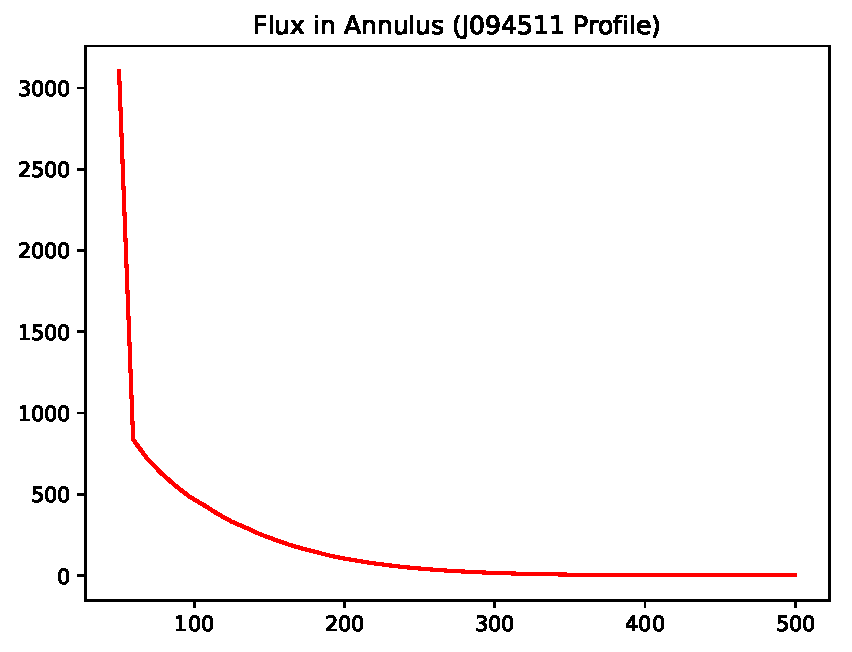
\includegraphics[width=0.32\textwidth]{J094511_R_annulus_flux.eps}
    \caption{Radial profile of J094511 in the Sloan $u'g'r'$ bands.}
    \label{fig:radial_profiles}
\end{figure}

This profile, unsurprisingly, also takes a Gaussian form. In order to determine whether there is a contribution $F_b$ from an intervening source, we can compare this profile to that of other point sources (stars) in the frame. The point-spread-function (PSF) of a CCD is the reponse of the pixel array to a point source in the frame.\cite{photutils_psf}\cite{anderson_2000} By normalising the profile of an intragalactic point source in the frame to its maximum, I can obtain a reasonable form for the PSF of the LT.

If there is \textit{not} an intervening galaxy in the field of J094511, we would expect its normalised profile to have the same form as the LT PSF. If, however, there is a diffuse but faint intervening source, the contribution $F_b$ from this source should be measurable in the profile of J094511 as excess flux in the ``wings'' of the Gaussian. The PSF can then be subtracted from the normalised profile of J094511 to obtain a profile for the intervening galaxy or dwarf galaxy.

Unfortunately, I did not have time to perform these calculations with rigor, but the existing codebase should be sufficient to acquire this profile, only by specifying the proper coordinates of another point source in the frame.

\section{Conclusion}

In summary, I have developed two main methods for aligning and stacking frames to increase the S/N ratio of faint objects in the LT data: whole pixel alignment and stacking using WCS information in the FITS header, and stacking of resampled Gaussian functions fitted to individual frames. Several advantages of Gaussian fitting/resampling over whole pixel stacking are demonstrated, and the resulting stacks used to extract flux profiles for J094511, a hypervariable AGN. The codebase for this is robust and extendable, and could with little modification be used to centroid, align, stack, and extract flux profiles for any object specified by its known equatorial coordinates. The profiles which were extracted appear to be in broad agreement with those extracted by Bruce et al. 2002, but further investigation is needed to verify this, and to verify the presence of excess luminosity in the wings of the profile. If confirmed, the presence of a flux contribution $F_b$ from an intervening galaxy is a strong argument for microlensing events as an explanation for this AGN's hypervariability, rather than tidal instability in the accretion disk.

\section*{Acknowledgements}

Special thanks to Andy Lawrence, professor at the Royal Observatory Edinburgh, for his support and advice throughout this project. Thanks also to James Goodman\footnote{\url{github.com/SlothInABox}}, a fellow undergraduate at the University of Edinburgh, who worked tirelessly with me to develop the original \textsc{fits-utils} module, much of which has been repurposed for this project. Thanks to Patrick Smith, for cultivating in me a love of empiricism in my formative school years. And finally, thanks to my father, who even before I could stand, took me for walks under the stars.

\printbibliography

\end{document}
